\section{本周工作}
\begin{frame}{本周工作}
    \begin{columns}
        \column{0.5\textwidth}
        \begin{figure}
            \centering
            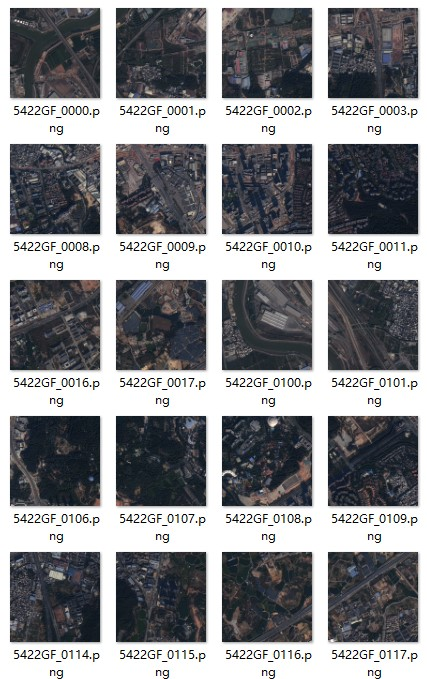
\includegraphics[height=6cm]{pic/pic0101.jpg}
            \caption{数据集}
            \label{fig:0101}
        \end{figure}

        \column{0.5\textwidth}
        \begin{itemize}
            \item 制作十倍超分数据集         
            \item 训练meta-SR scale=10.0超分模型
        \end{itemize}
    \end{columns}
\end{frame}

\section{实验结果}
\begin{frame}{实验结果}
    \begin{figure}
        \centering
        
\includegraphics[width=11cm]{pic/pic0102.jpg}
        \caption{LR\quad x4x2.5\quad x5x2 \quad x10 \quad HR}
        \label{fig:0102}
    \end{figure} 

    \begin{table}[h]
        \centering
        \begin{tabular}{ m{1.5cm} | m{1.5cm} | m{1.5cm} | m{1.5cm} | m{1.5cm}}
            \hline
             & LR & x4.0x2.5 & x5.0x2.0 & x10.0 \\ \hline
            ssim & 00.47 & 00.37 & 00.38 & 00.49 \\ \hline       
            pnsr & 22.29  & 17.09 & 17.33 & 22.35\\ \hline           
        \end{tabular}
        \caption{ssim and pnsr}
    \end{table}
\end{frame}

% \begin{frame}{数据总览}
%     \begin{figure}[!htbp]
%         \centering
%         \subfloat[{\tiny gf1-s2}]{\label{fig:0101a}
%         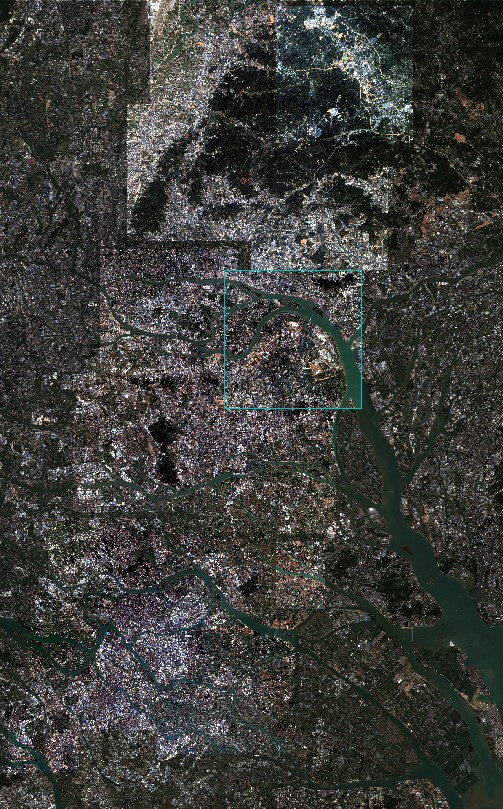
\includegraphics[height=5.5cm]{pic/pic0101gf1.jpg}}
%         \quad
%         \subfloat[{\tiny gf2-s2}]{\label{fig:0101b}
%         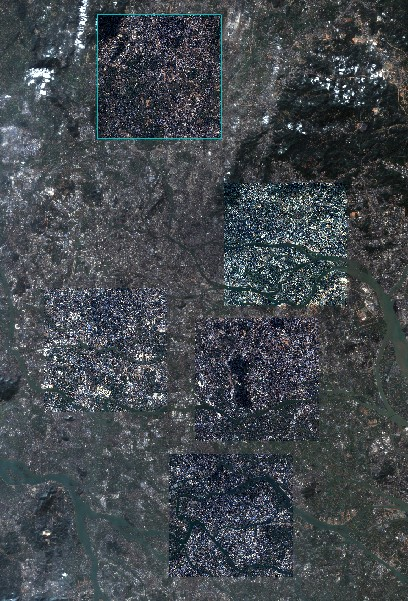
\includegraphics[height=5.5cm]{pic/pic0101gf2.jpg}}
%         \caption{{\tiny GF-S2数据集}}
%         \label{fig:0101}
%     \end{figure}
% \end{frame}

% \begin{frame}{数据集整理}
%     \begin{figure}
%         \centering
%         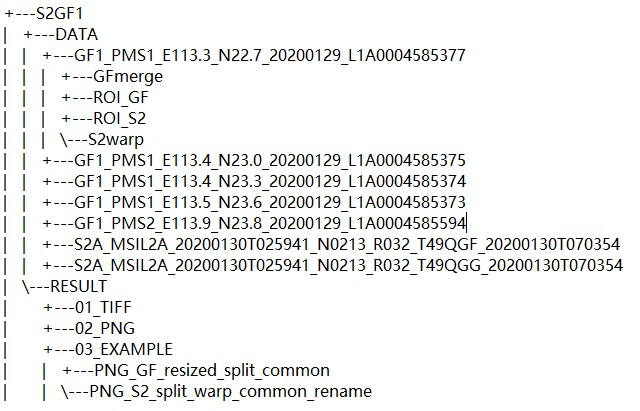
\includegraphics[width=10cm]{pic/pic0102gf1.jpg}
%         \caption{GF1-S2数据集结构}
%         \label{fig:0102a}
%     \end{figure}
% \end{frame}

